\documentclass[a4paper,11pt]{article}

% Use utf-8 encoding for foreign characters
\usepackage[utf8]{inputenc}
\usepackage[british,english]{babel}
\usepackage[T1]{fontenc}

% Setup for fullpage use
\usepackage{fullpage}

% Multipart figures
\usepackage{subfigure}

% More symbols
\usepackage{amsmath}
\usepackage{amssymb}
\usepackage{latexsym}

% For pretty URLs, see: http://en.wikibooks.org/wiki/LaTeX/Hyperlinks
\usepackage{hyperref}

% Surround parts of graphics with box
\usepackage{boxedminipage}

% Package for including code in the document
\usepackage{listings}

% If you want to generate a toc for each chapter (use with book)
\usepackage{minitoc}

% Uncomment if you want to use Palatino as font
\usepackage[sc]{mathpazo}
\linespread{1.05}         % Palatino needs more leading (space between lines)

% This is now the recommended way for checking for PDFLaTeX:
\usepackage{ifpdf}


\addto\captionsenglish{\renewcommand{\refname}{}}

%\newif\ifpdf
%\ifx\pdfoutput\undefined
%\pdffalse % we are not running PDFLaTeX
%\else
%\pdfoutput=1 % we are running PDFLaTeX
%\pdftrue
%\fi

\ifpdf
\usepackage[pdftex]{graphicx}
\else
\usepackage{graphicx}
\fi
\title{Deliverable 4: Sprint \#1\\\small{for}\\\small{Danske Bank: Peer-to-peer}}
\author{ Group Delta:\\Jesper Borgstrup, Thomas Kjeldsen and Mads Ohm Larsen }

\date{April 1, 2011}

\begin{document}

\ifpdf
\DeclareGraphicsExtensions{.pdf, .jpg, .tif}
\else
\DeclareGraphicsExtensions{.eps, .jpg}
\fi

\maketitle

%\tableofcontents
%\vspace{2cm}

\section{Requirements for this deliverable}
\begin{enumerate}
\item Doing a demo in class (on 2011-03-30)
\item Giving us access to your source code
\item Handing in a collection of your sprint material
\item Describing a sprint retrospective (e.g., as a set of bullets outlining what
when well, what went wrong, and how you will improve for the next sprint)
\end{enumerate}

The Sprint Demo was given on March 9th. This document describes requirements 2-4 as well as the sprint learning goal -- software design and architecture.

\section{Software design and architecture}
Although our software currently is implemented as a standalone application, we intend, for our third sprint, to divide the functionality into two parts:
\begin{itemize}
\item An independent library responsible for establishing a secure bluetooth connection between two phones aided by an initial out-of-band (OOB) connection such as Bump.
\item A sample application utilizing the library to securely send arbitrary files (e.g. pictures, video or music) to another nearby device using the aforementioned bluetooth connection.
\end{itemize}

\paragraph{Identity providers}
An OOB connection used to exchange bluetooth identity information to setup the actual connection will be known as an \emph{identity provider}. In order to seamlessly support multiple identity providers, we plan on using the Abstract Factory\cite{GangOfFour} pattern. This way, a user of the API will not have to know about or rely upon the implementations of the different identity providers, but simply decide which provider to use.

\paragraph{Android Intents}
Luckily, parts of the Android API seems to have been designed with some design patterns in mind. As such, the Android intent system seems inspired by the Command\cite{GangOfFour} pattern with which you encapsulate all the information needed the call a method when appropriate, so the system asynchronously can call the method.

\section{Source code access}
Our source code is publicly available on Github from \url{https://github.com/omegahm/DBP2P}.

Please note that we are working on multiple branches (use the button switch branch to view another branch).

The master branch currently holds only documentation and deliverables, while we have a dedicated development branch for sprint \#1 named \texttt{dustytuba}.

If you wish to checkout our code (read-only) using Git, then use git clone with this URL:
\url{git://github.com/omegahm/DBP2P.git}


\section{Sprint material}
%TODO
Sprint Material needed to assess our progress include the following:
\begin{itemize}
\item source code (version number and access method is sufficient)
\item product backlog (before and after the sprint)
\item sprint backlog
\item any other material (e.g., burndown chart) that illustrates your progress
\end{itemize}

% TODO: Describe Acunote in general and that access have been granted.

\subsection{Source Code}

%The final product of sprint \#1 has been merged into the master branch as per commit-id  \href{https://github.com/omegahm/DBP2P/commit/1abf2360b074729c7f2eefacb294f21fb668f9db}{1abf2360b074729c7f2eefacb294f21fb668f9db}.

%The code and tests are located in the folders ``DustyTuba'' and ``DustyTuba''.

The following tasks have been completed during this sprint:
\begin{itemize}
	\item item
\end{itemize}

%In regards to our user stories, the tasks completed corresponds to the following user stories:
%\begin{verbatim}
%  As a        user
%  I want to   identify a nearby device
%  Such that   I can establish a connection in order to transfer information safely	
%
%  As a        user
%  I want to   identify a nearby device using Bump
%  Such that   I can establish a connection in order to transfer information safely
%\end{verbatim}

\subsection{Product Backlog}

%\begin{figure}[ht!]
%	\begin{center}
%	% Insert sprint backlog here
%	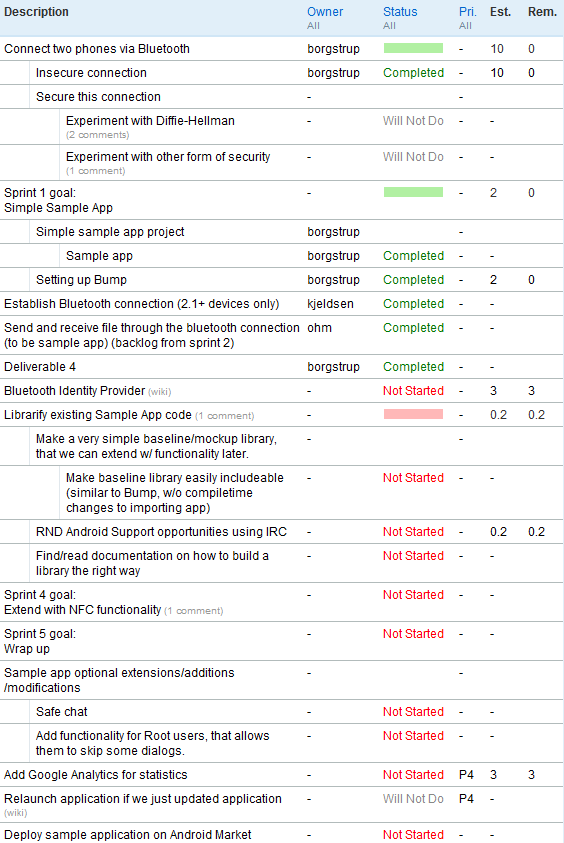
\includegraphics[width=1.4\textwidth, angle=-90]{productbacklog.png}		
%	\end{center}
%	\caption{Our product backlog at the end of sprint \#1.}
%	\label{productbacklog}
%\end{figure}

\subsection{Sprint Backlog}
%Our sprint backlog is shown in figure \ref{sprintbacklog} on page \pageref{sprintbacklog}.

%\begin{figure}[ht!]
%	\begin{center}
%	% Insert sprint backlog here
%	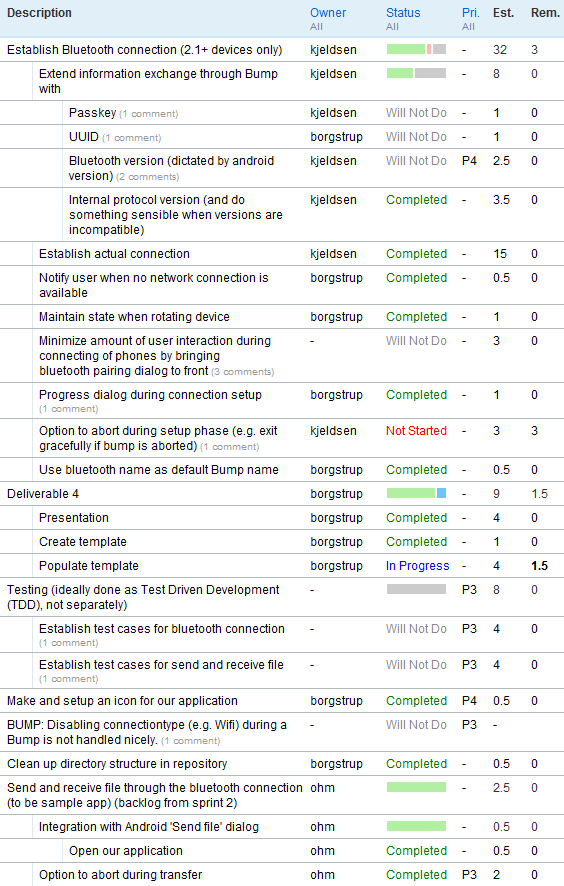
\includegraphics[width=1.4\textwidth, angle=-90]{sprintbacklog.png}		
%	\end{center}
%	\caption{Our sprint backlog after the sprint was finished}
%	\label{sprintbacklog}
%\end{figure}

\subsection{Burndown chart}

%Our burndown chart is shown in figure \ref{burndown} on page \pageref{burndown}.

%\begin{figure}[ht!]
%	\begin{center}
%	% Insert burndown chart here
%	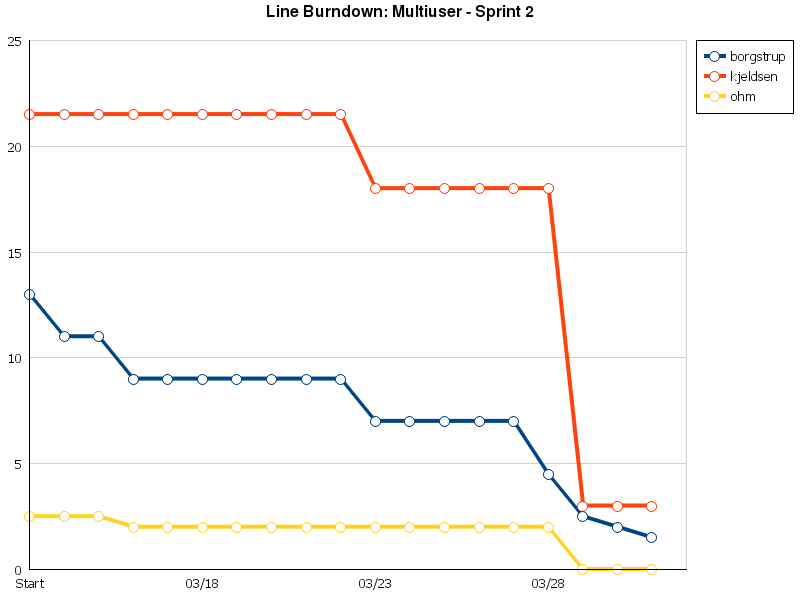
\includegraphics[width=\textwidth]{burndown.png}		
%	\end{center}
%	\caption{Our burndown chart at the end of the sprint}
%	\label{burndown}
%\end{figure}

\subsection{Other relevant material}
%We have got an Acunote account\footnote{\url{http://dbp2p.acunote.com/}} setup, and access to this have been granted.

%\clearpage
\section{Sprint retrospective}

What went well during this sprint:

\begin{itemize}
	\item item
\end{itemize}

\noindent
What went wrong:

\begin{itemize}
	\item item
\end{itemize}

\noindent
How we will improve:
\begin{itemize}
	\item item
\end{itemize}

\section{References}
\begin{thebibliography}{9}
\vspace{-3em}

\bibitem{GangOfFour}
  Gamma et al.,
  \emph{Design Patterns: Elements of Reusable Object-Oriented Software}.
  Addison Wesley, 1994.

\end{thebibliography}

\end{document}
